\documentclass[11pt]{report}

\usepackage[margin=0.5in]{geometry}

\usepackage{graphicx} % Add pictures to your document
\usepackage{float}
\usepackage{listings}
\usepackage{xcolor}
\usepackage{pgfplots}
\lstset { %
    language=C,
    backgroundcolor=\color{black!5}, % set backgroundcolor
    basicstyle=\footnotesize,% basic font setting
}

\begin{document}

\title{\huge{\textbf{RCOM TP1}} \\ Turma 3 // Grupo 3 \\ RCOM 2020/2021 \\ MIEIC FEUP}
\author{João de Jesus Costa \\ \texttt{up201806560} \and
	João Lucas Silva Martins \\ \texttt{up201806436}}
\date{\today{}}

\begin{figure}[b]
	\centering
	
\includegraphics[width=0.6\textwidth]{feup_logo.png}
\end{figure}
\maketitle{}

\tableofcontents{}
\newpage

\chapter{Sumário}
// TODO

{\let\clearpage\relax \chapter{Introdução}}
Este relatório incide sobre o projecto desenvolvido para a unidade curricular
de RCOM. Neste projecto foi pedido o desenvolvimento de uma aplicação, em
linguagem C, que permitisse o envio de ficheiros, entre dois computadores,
através de uma \textit{serial port}.

Além disso, esta aplicação devia estar organizada em camadas independentes
(discutidas mais à frente) e deve ser resistente a ruído e desconexão durante
o envio de informação.

// TODO Dizer o q cada chapter tem

{\let\clearpage\relax \chapter{Arquitetura}}

O código encontra-se dividido em duas partes principais: a camada de aplicação e
a camada de ligação de dados. Por sua vez, estas duas camadas dividem-se na sua
componente pública, que é utilizada por um agente externo (\textbf{interface}), e a sua
componente privada que integra as funções internas da camada.

{\let\clearpage\relax \chapter{Estrutura do código}}

\section{Camada de aplicação}

A API da camada de aplicação é implementada nos ficheiros \textit{app\_layer.h}
e \textit{app\_layer.c}. Para utilizar esta camada é necessário instanciar um objeto
\textbf{struct applicationLayer}.

\begin{lstlisting}
struct applicationLayer {
  int fd;  /* file descriptor correspondente a porta serie */
  enum applicationStatus status;  /* TRANSMITTER or RECEIVER */
  char file_name[256];  /* name of file to transmit (if any) */
  long file_size;       /* size of file to transmit (if any) */
  long chunksize;       /* tansmission chunksize */
};
\end{lstlisting}

A função \textbf{initAppLayer} inicia um objeto do tipo \textbf{struct applicationLayer}
e a sua correspondente \textbf{struct linkLayer}.
\begin{lstlisting}
void initAppLayer(struct applicationLayer *appLayer, int baudrate,
                  long chunksize);
\end{lstlisting}

A função \textbf{llopen} abre uma conexão na dada \textit{serial port}.
\begin{lstlisting}
int llopen(int porta, enum applicationStatus appStatus);
\end{lstlisting}

A função \textbf{llwrite} envia o dado \textit{buffer} através da ligação pré estabelicida.
\begin{lstlisting}
int llwrite(int fd, char *buffer, int length);
\end{lstlisting}

A função \textbf{llread} recebe um pacote da ligação pré-estabelecida para \textit{buffer}.
\begin{lstlisting}
int llread(int fd, char **buffer);
\end{lstlisting}

A função \textbf{llclose} fecha uma ligação anteriormente estabelecida.
\begin{lstlisting}
int llclose(int fd, enum applicationStatus appStatus);
\end{lstlisting}

A função \textbf{sendFile} lê e envia o ficheiro especificado pela camada de aplicação.
\begin{lstlisting}
int sendFile(struct applicationLayer *appLayer);
\end{lstlisting}

A função \textbf{sendFile} recebe o conteúdo de um ficheiro transmitido à camada de aplicação,
guardando-o em \textit{res}.
\begin{lstlisting}
int receiveFile(struct applicationLayer *appLayer, unsigned char **res);
\end{lstlisting}

A função \textbf{write\_file} cria um ficheiro com o conteúdo de \textit{file\_content}
e com nome especificado pela camada de aplicação.
\begin{lstlisting}
void write_file(struct applicationLayer *appLayer, unsigned char *file_content);
\end{lstlisting}

\section{Camada de ligação}

A API da camada de ligação é definida nos ficheiros \textit{data\_link.h} e
\textit{data\_link.c}. Para utilizar esta camada é necessário instanciar um objeto
do tipo \textbf{struct linkLayer}.

\begin{lstlisting}
struct linkLayer {
  char port[20];                 /* Dispositivo /dev/ttySx, x = 0, 1 */
  int baudRate;                  /* Velcidade de transmissao */
  unsigned int sequenceNumber;   /* Numero de sequencia da trama: 0, 1*/
  unsigned int timeout;          /* Valor do temporizador, e.g.: 1 sec */
  unsigned int numTransmissions; /* Numero de retransmissoes em caso de falha */
  vector *frame;
};
\end{lstlisting}

A função \textbf{initLinkLayer} inicializa uma camada de ligação e o seu respetivo \textbf{vector}.
\begin{lstlisting}
struct linkLayer initLinkLayer();
\end{lstlisting}

A função \textbf{initConnection} estabelece uma conexão do tipo indicado em \textit{isReceiver}
na camada de ligação dada.
\begin{lstlisting}
int initConnection(struct linkLayer *linkLayer, int fd, bool isReceiver);
\end{lstlisting}

A função \textbf{endConnection} fecha uma conexão do tipo indicado em \textit{isReceiver}
na camada de ligação dada.
\begin{lstlisting}
int endConnection(struct linkLayer *linkLayer, int fd, bool isReceiver);
\end{lstlisting}

A função \textbf{getFrame} recebe uma trama através de uma conexão pré-estabelecida.
\begin{lstlisting}
int getFrame(struct linkLayer *linkLayer, int fd, unsigned char **packet);
\end{lstlisting}

A função \textbf{getFrame} envia uma trama para uma conexão pré-estabelecida com o tamanho
\textit{len}.
\begin{lstlisting}
int sendFrame(struct linkLayer *linkLayer, int fd, unsigned char *packet,
              int len);
\end{lstlisting}

{\let\clearpage\relax \chapter{Casos de usos principais}}

A nossa solução para a proposta de trabalho contempla dois casos de uso: o envio de um ficheiro
como emissor e a receção do mesmo como recetor. Este modo de funcionamento deve ser referido
na chamada do programa através da flag \textit{-s RECEIVER} ou \textit{-s TRANSMITTER}.

Para o programa ser executado como recetor é obrigatório especificar o número da porta série a usar.



Se o programa for executado como emissor, será necessário especificar o caminho para o ficheiro a enviar,
em adição aos outros argumentos já enunciados anteriormente. Enquanto emissor, também pode ser útil referir
o \textit{chunksize} a usar.

\chapter{Protocolos}

\section{Protocolo de ligação lógica}

Este protocolo e responsável pela preparação da informação a enviar pela
\textit{serial port} e os mecanismos de recuperação de erros/falhas.

A informação é transmitida em tramas. Existem três tipos de tramas:
\textbf{informação, supervisão, e não numeradas}. As tramas de informação
carregam os dados a enviar. As tramas de supervisão indicam se um dada de
trama de informação foi bem (ou mal) recebida. As tramas não numeradas servem
para implementar os mecanismos de inicio e conclusão de uma conexão.

As tramas começam e terminam por um byte de \textit{flag} (0x7E) e são
identificadas por um bit de sequência que oscila entre 0 e 1. Este bit é útil
para que o protocolo consiga garantir que nenhuma trama foi perdida ou repetida.

De modo a garantir que o byte correspondente à \textit{flag} (byte que indica
o inicio e o final de um trama) não ocorre no campo de informação ou no BCC,
é realizado o byte \textit{stuffing} (e consequentemente \textit{destuffing})
destas.
\begin{lstlisting}
int stuffByte(unsigned char byte, unsigned char res[]) {
  int bytes_returned = 1;
  if (byte == ESC) {
    res[0] = ESC;
    res[1] = ESC ^ STUFF_BYTE;
    bytes_returned = 2;
  } else if (byte == FLAG) {
    res[0] = ESC;
    res[1] = FLAG ^ STUFF_BYTE;
    bytes_returned = 2;
  } else
    res[0] = byte;
  return bytes_returned;
}

int stuffString(unsigned char *str, unsigned char *res, int size) {
  int j = 0;
  for (int i = 0; i < size; ++i) {
    unsigned char stuffedBytes[2];
    int n = stuffByte(str[i], stuffedBytes);
    res[j++] = stuffedBytes[0];
    if (n > 1)
      res[j++] = stuffedBytes[1];
  }
  return j;
}

unsigned char destuffByte(unsigned char byte) { return byte ^ STUFF_BYTE; }
\end{lstlisting}

O cabeçalho de cada trama é protegido por um BCC. As tramas de informação têm um
segundo BCC que protege a informação transmitida.
\begin{lstlisting}
unsigned char calcBCC2Field(unsigned char *buf, int size) {
  unsigned char ret = 0;
  for (int i = 0; i < size; ++i)
    ret ^= buf[i];
  return ret;
}

bool checkBCC2Field(unsigned char *buf, int size) {
  return calcBCC2Field(buf, size) == buf[size];
}
\end{lstlisting}

Este protocolo faz uso de uma máquina de estados de modo a conseguir interpretar
os bytes recebidos. Esta interpretação facilita o \textit{byte destuffing}, a
recuperação de erros e a identificação do final de tramas.
\begin{lstlisting}
/* STATE MACHINE */
typedef enum {
  FLAG_RCV = 0,
  A_RCV = 1,
  CI_RCV = 2,
  CS_RCV = 3,
  BCC_RCV = 4,
  OTHER_RCV = 5
} transitions;

typedef enum {
  START_ST = 0,
  FLAG_ST = 1,
  A_ST = 2,
  CS_ST = 3,
  BCC_ST = 4,
  CI_ST = 5,
  D_ST = 6,
  STOP_ST = 7
} state;

static state state_machine[][6] = {
/*  F_RCV     A_RCV     CI_RCV    CS_RCV    BCC_RCV   OTHER_RCV */
  { FLAG_ST,  START_ST, START_ST, START_ST, START_ST, START_ST},  // START_ST
  { FLAG_ST,  A_ST,     START_ST, START_ST, START_ST, START_ST},  // FLAG_ST
  { FLAG_ST,  START_ST, CI_ST,    CS_ST,    START_ST, START_ST},  // A_ST
  { FLAG_ST,  START_ST, START_ST, START_ST, BCC_ST,   START_ST},  // CS_ST
  { STOP_ST,  START_ST, START_ST, START_ST, START_ST, START_ST},  // BCC_ST
  { FLAG_ST,  START_ST, START_ST, START_ST, D_ST,     START_ST},  // CI_ST
  { STOP_ST,  D_ST,     D_ST,     D_ST,     D_ST,     D_ST    },  // D_ST
  { STOP_ST,  STOP_ST,  STOP_ST,  STOP_ST,  STOP_ST,  STOP_ST }   // STOP_ST
};
\end{lstlisting}

\section{Protocolo de aplicação}

Este protocolo é responsável por abrir a porta série, ler/escrever o ficheiro
transferido. Para isso, inicia a camada de ligação de dados, faz a segmentação
do ficheiro a transmitir, interpreta a informação recebida e escreve a
informação para o ficheiro resultante.

Os pacotes destes protocolo possuem um cabeçalho que indica o tipo de mensagem
que contém: controlo (tamanho ficheiro e nome do ficheiro) ou bloco de
informação. No caso dos pacotes de informação, o cabeçalho contém um byte
de sequência que indica a ordem dos pacotes, começando em zero. A cada pacote
recebido este número deve aumentar por um e voltar a zero após o número 255.
Se esta não for comprida, é evidente que ocorreu um erro grave e que a execução
deve ser terminada.

No lado do emissor, o ficheiro é lido e, em seguida, enviado em blocos de
tamanho \textit{chunksize} bytes (valor configurável). No lado do recetor, o
ficheiro é lido em blocos de tamanho \textit{chunksize} definido pelo emissor.
Quando a transmissão termina, a informação lida é escrita no ficheiro.

O primeiro e último pacotes transmitidos pelo protocolo são pacotes de controlo.
Estes pacotes contém informação relativa ao nome do ficheiro e o seu tamanho e
um byte identificador. Estes dois pacotes devem ser idênticos, à excepção do byte
identificador (um sinalizará o inicio e o outro o fim da transmissão).

{\let\clearpage\relax \chapter{Validação}}

De modo a validar o correto funcionamento do programa, enviamos diversos ficheiros
com tamanhos e formatos distintos, fazendo variar o valor do \textit{baudrate}
e do \textit{chunksize} (este afecta o tamanho das tramas).

Fizemos três tipos de envios: envios sem introdução de erros, envios com cortes
na ligação, e envios com erros aleatorios (nomeadante no BCC do cabeçalho).

// TODO mostrar prints do prog

\chapter{Eficiência do protocolo de ligação de dados}

\subsection{Tempo de propagação}

Com o objetivo de medir de forma fiável a eficiência do protocolo, foi calculado
o tempo de propagação $T_{prop}$ através da fórmula
$T_{prop} = T_{absRecebido} - T_{absEnviado}$. Sendo $T_{absRecebido}$ e $T_{absEnviado}$ o tempo
absoluto de envio do byte de teste, e o tempo de receção do byte de teste, respetivamente.

\begin{table}[h!]
  \begin{center}
    \caption{Cálculo do tempo de propagação médio}
    \label{tab:table1}
    \begin{tabular}{l|c|r|r} % <-- Alignments: 1st column left, 2nd middle and 3rd right, with vertical lines in between
        \textbf{$T_{absEnviado}(ns)$} &\textbf{$T_{absRecebido}(ns)$} & \textbf{$T_{prop}(ns)$} & \textbf{$\mu T_{prop}$}\\
      \hline
      267368335 & 264536179 & 2832156\\
      469990377 & 467159729 & 2830648\\
        672241506 & 669431417 & 2810089 & 2819355\\
      874435168 & 871625091 & 2810077\\
      77204397 & 74385042 & 2819355\\
    \end{tabular}
  \end{center}
\end{table}

\subsection{Análise de eficiência}

De modo a obter resultados mais precisos foram efetuados três medições
para cada cálculo do tempo de execução. As medições foram feitas remotamente
nos computadores laboratoriais da sala I320. Em cada medição foi usado um
\textit{chunksize} de 256 Bytes e o ficheiro usado foi o fornecido pelo moodle (pinguim.gif).
\begin{table}[h!]
  \begin{center}
    \caption{Cálculo da eficiência sem introdução de erros}
    \label{tab:table1}
    \begin{tabular}{l|r} % <-- Alignments: 1st column left, 2nd middle and 3rd right, with vertical lines in between
        Baudrate & \textbf{$  T_{execucao} (s) $} \\
      \hline
        9600 & 12.23109\\
        19200 & 6.11795\\
        38400 & 3.06131\\
        57600 & 2.04245\\
        115200 & 1.02359\\
    \end{tabular}
  \end{center}
\end{table}

\begin{table}[h!]
  \begin{center}
    \caption{Cálculo da eficiência com introdução de erros}
    \label{tab:table1}
    \begin{tabular}{l|c|c|c} % <-- Alignments: 1st column left, 2nd middle and 3rd right, with vertical lines in between
        Baudrate & \textbf{$  T_{execucao} (s) $} & Nº pacotes enviados & Nº pacotes reenviados \\
      \hline
        9600 & 15.11709 & 60.00000 & 12.00000\\
        19200 & 7.11741 & 56.00000 & 8.00000\\
        38400 & 4.08493 & 63.00000 & 15.00000\\
        57600 & 2.55259 & 59.33333 & 11.33333\\
        115200 & 1.43659 & 68.00000 & 20.00000\\
    \end{tabular}
  \end{center}
\end{table}

\begin{table}[h!]
  \begin{center}
    \caption{Cálculo da eficiência com variação do chunksize}
    \label{tab:table1}
    \begin{tabular}{l|r} % <-- Alignments: 1st column left, 2nd middle and 3rd right, with vertical lines in between
        Chunksize & \textbf{$  T_{execucao} (s) $} \\
      \hline
        1 & 58.20041\\
        10 & 8.42766\\
        100 & 3.44801\\
        1000 & 2.94857\\
        10000 & 2.90310\\
    \end{tabular}
  \end{center}
\end{table}

\chapter{Graphs}
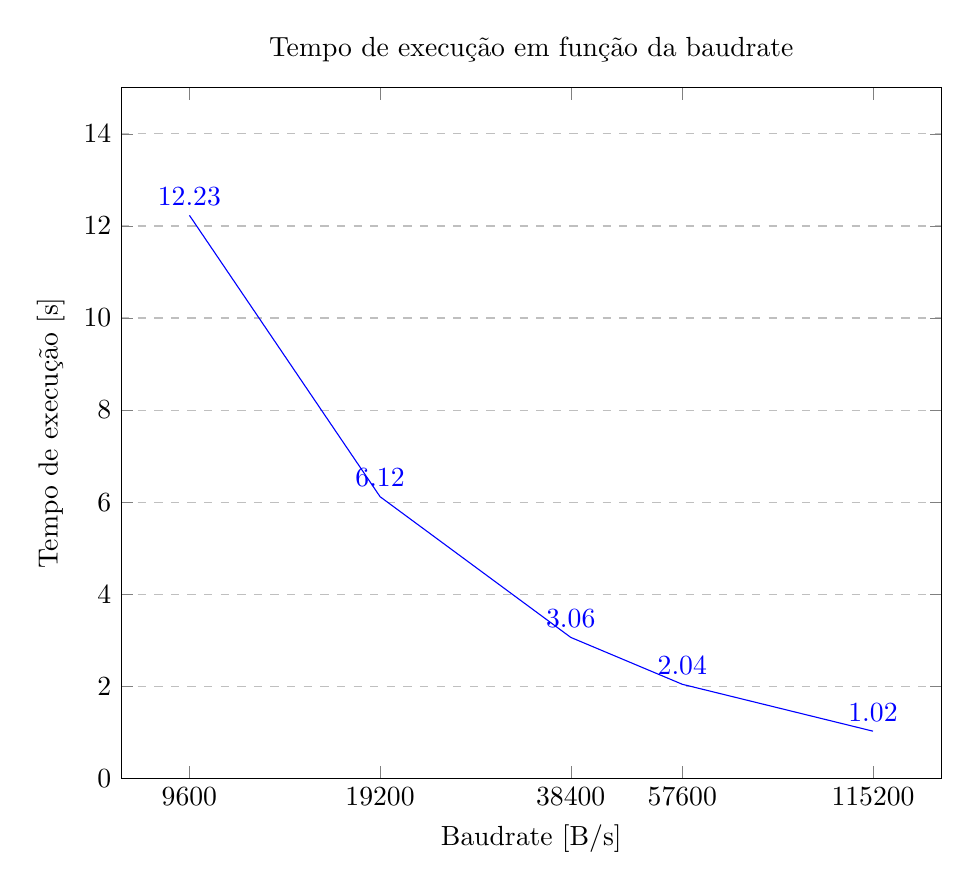
\begin{tikzpicture}
\begin{axis}[
    title={Tempo de execução em função da baudrate},
    width=12cm,
    xlabel={Baudrate [B/s]},
    ylabel={Tempo de execução [s]},
    ymin=0, ymax=15,
    xmode=log,
    xtick={9600, 19200, 38400, 57600, 115200},
    xticklabels={9600, 19200, 38400, 57600, 115200},
    legend pos=north west,
    ymajorgrids=true,
    grid style=dashed,
    nodes near coords,
]

\addplot[
    color=blue,
    ]
    coordinates {
        (9600, 12.23109)
        (19200, 6.11795)
        (38400, 3.06131)
        (57600, 2.04245)
        (115200, 1.02359)
    };
\end{axis}
\end{tikzpicture}

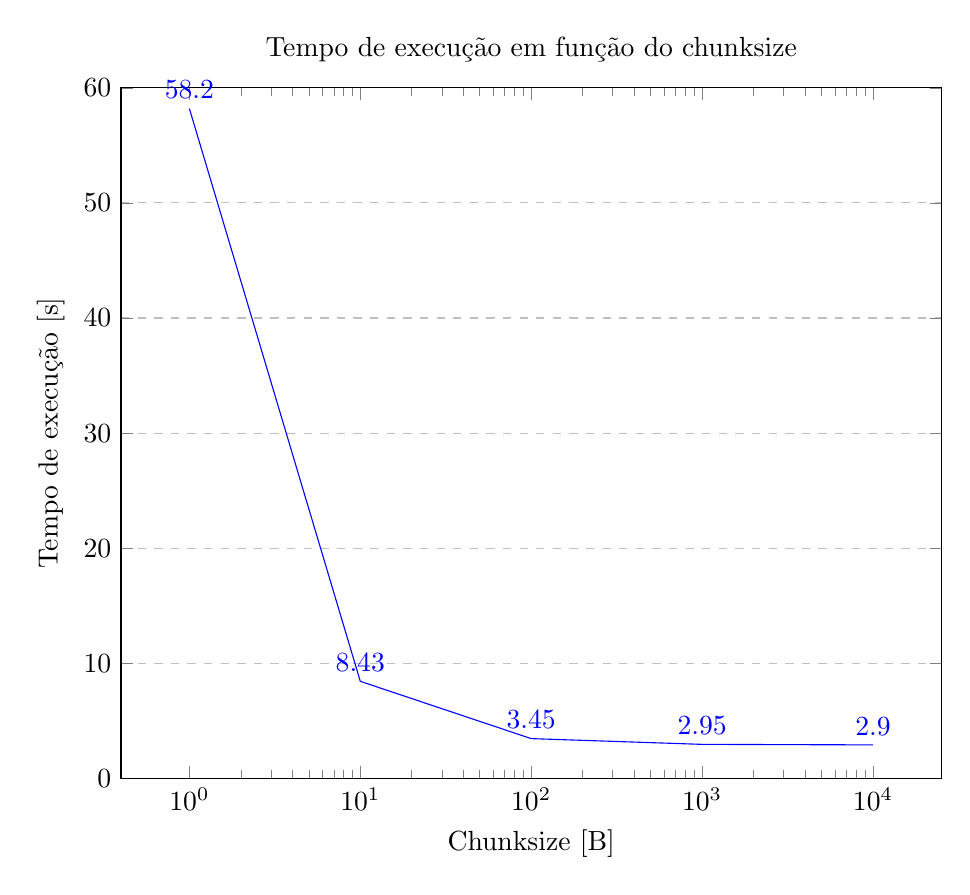
\begin{tikzpicture}
\begin{axis}[
    title={Tempo de execução em função do chunksize},
    width=12cm,
    xlabel={Chunksize [B]},
    ylabel={Tempo de execução [s]},
    ymin=0, ymax=60,
    xmode=log,
    xtick={1, 10, 100, 1000, 10000},
    legend pos=north west,
    ymajorgrids=true,
    grid style=dashed,
    nodes near coords,
]

\addplot[
    color=blue,
    ]
    coordinates {
        (1 , 58.20041)
        (10 , 8.42766)
        (100 , 3.44801)
        (1000 , 2.94857)
        (10000 , 2.90310)
    };
\end{axis}
\end{tikzpicture}

\chapter{Conclusões}

\end{document}
